\chapter{PROPOSTA EXPERIMENTAL}
\label{chp:experiments}

Para o estudo em questão, propõe-se três experimentos. Os objetivos e a descrição detalhada de cada um destes experimentos estão nas seções a seguir.


\section{Definição do modelo do comparador}
\label{sec:experiments:emb-comparator}
O objetivo desse experimento é definir os parâmetros do comparador de \textit{embeddings}. Os parâmetros utilizados, bem como os valores para cada um neste experimento, se encontram na lista abaixo.

\begin{itemize}
    \item topologias: \gls{resnet} e \gls{mlp}
    \item número de camadas escondidas: 2, 4, 6 e 8
    \item função de ativação: \gls{tanh} e \gls{relu}
    \item \textit{dropout}: 5, 10, 15 e 20
    \item regularização L1 e L2: 0.001, 0.01 e 0.1
\end{itemize}

Vale frisar que tais valores foram escolhidos de forma empírica, durante a concepção desse experimento. 

Além disso, para variar os valores no modelo de comparação, é necessário que os \textit{encoders} de código-fonte e texto estejam fixos. Com isso, para este experimento, foi escolhido, de forma empírica, o par de \textit{encoders} código-fonte/texto \textit{CodeBERT} e \textit{BERT}.

\section{Comparação entre \textit{encoders}}
\label{sec:experiments:encoders}
Com os parâmetros do comparador de \textit{embeddings} definidos pelo experimento \ref{sec:experiments:emb-comparator}, este experimento será realizado para comparar pares de \textit{embeddings} de diferentes \textit{encoders}. Para tanto, foram escolhidos seis \textit{encoders}, conforme mostra a \ref{fig:experiments-encoders}.

\begin{figure}[htbp]
    \centering
        \caption{\textit{Encoders} selecionados}
        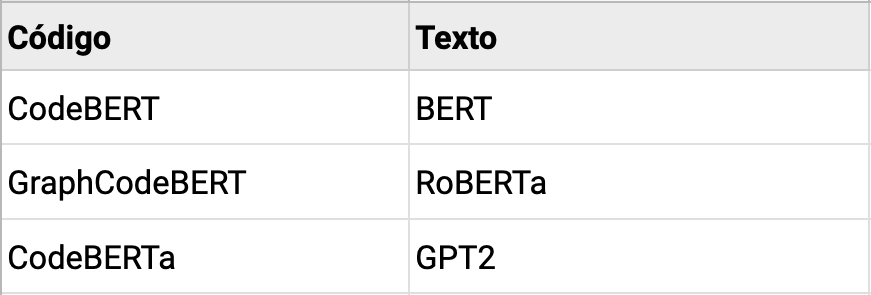
\includegraphics[scale=0.5]{resources/images/metodologia/encoders-list.png}
        \smallcaption{Fonte: Autor.}
        \label{fig:experiments-encoders}
\end{figure}

Com isso, 8 pares de \textit{encoders} serão utilizados nesse experimento; isso porque um par de \textit{encoder} já foi utilizado no primeiro experimento, eliminando, portanto, a necessidade de utilizá-lo novamente. A ideia central desse experimento é analisar como que o modelo de comparação se comporta com diferentes topologias de \textit{encoders}, e seus respectivos \textit{embeddings}.

\section{Generalização dos \textit{encoders}}
\label{sec:experiments:generic_encoder}
Por fim, o objetivo desse experimento é avaliar se o modelo de comparação é capaz de abstrair os \textit{encoders} utilizados no sistema.

Para tanto, será criada uma base de pares de \textit{embeddings} código-fonte/texto. Tais \textit{embeddings} serão gerados a partir de todos os nove pares possíveis formados pelos \textit{encoders} da figura \ref{fig:experiments-encoders}. Então, será realizado apenas um treinamento com todos os pares de \textit{embeddings} da base.

Com isso, a hipótese desse experimento é que se o modelo de comparação obtiver bons resultados nesse cenário, então este é capaz de abstrair os \textit{encoders} utilizados para geração dos \textit{embeddings}. Em outras palavras, dado quaisquer pares de \textit{encoders} (formados pelos \textit{encoders} da figura \ref{fig:experiments-encoders}) código-fonte/descrição, o modelo de comparação será capaz de determinar a similaridade dos \textit{embeddings} gerados.
